\chapter{绪论}

\section{引言}
子痫前期(preeclampsia, PE)又名先兆子痫,是孕妇妊娠期特有的一种多系统进展性疾病, 与妊娠期高血压(gestational hypertension)、子痫(eclampsia)、
慢性高血压并发子痫前期(chronic hypertension with superimposed preeclampsia)以及妊娠合并慢性高血压(chronic hypertension)统称妊娠期
高血压疾病(hypertension disorders of pregnancy, HDP)\cite{OAG9,HDASOM,2000s1}。
子痫前期临床表现的显著特点是原发性高血压与蛋白尿。
近年来,组织的对子痫前期的涵盖范围进行了进一步的拓展,在妊娠20周后出现新发(原发)高血压,在两次间隔$4h$或$4h$以上的血压测定中,收缩压≥$140mmHg$和(或)
舒张压≥$90mmHg$,且伴有下列任一项或多项\cite{OAG9,FIGO}:
\begin{itemize}
    \item 孕妇出现蛋白尿症状,尿蛋白≥$300mg/24h$,或尿蛋白/肌酸酐比值≥$30mg/mol$,或随机尿蛋白≥(+);
    \item 孕妇无尿蛋白但伴有以下任一器官或系统功能紊乱、受累受损:心、肺(肺水肿)、肝(血清转氨酶水平为正常值2倍以上)、肾(血肌酐水平大于$1.1mg/dl$
    或为正常值2倍以上)等重要器官,或血液系统(血小板<$100 \times 10^{9}/L$)等)、消化系统、神经系统的异常改变等;
    \item 胎盘-胎儿受到累及:胎盘胎儿生长受限、脐动脉多普勒分析检测异常、死胎等。 
\end{itemize}

妊娠期高血压疾病可引起严重的母胎并发症,是孕产妇和围产儿病死率升高的主要原因\cite{OAG9}。
据世界卫生组织统计,子痫前期在孕妇中发病率高达5\%-10\%,是除体内大出血外孕妇死亡的第二大危险因素\cite{LCT2006},每年可导致全球范围内约76 000名孕妇死亡,并进一步导致约500 000
名胎儿/婴儿的死亡\cite{DAM2015,LCT2006}(如\autoref{fig:dhd}所示)。为推广普及人们对危及母婴生命安全的子痫前期的认知,同时教育女性了解她们当前及长期的健康风险,
全球孕妇保健组织自2017年起将每年的5月22日确定为世界子痫日(world preeclampsia day)(如\autoref{fig:wpd}所示)。
\begin{figure}[htb]
    \centering
    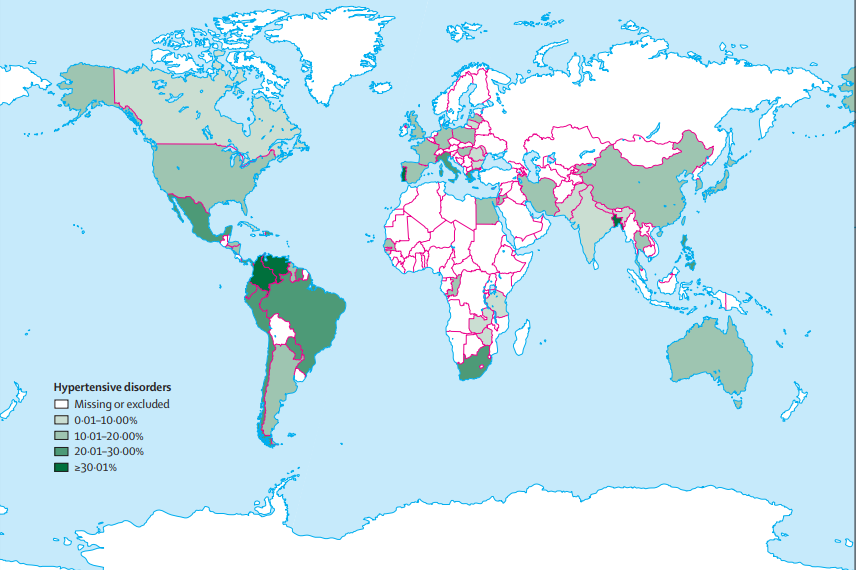
\includegraphics[width=.7\linewidth]{ch1/dhd}
    \caption{\label{fig:dhd}因妊娠期高血压疾病死亡孕妇的国家分布比例}
\end{figure}
\begin{figure}[htb]
    \centering
    
\includegraphics[width=.7\linewidth]{ch1/wpd}
    \caption{\label{fig:wpd}2021年世界子痫日主题:Preeclampsia: Beyond Pregnancy}
\end{figure}

就现阶段我国国情而言,由于人口基数大、人口出生率较高,导致每年妊娠孕妇数及新生儿数总量大。
同时,自全面开放二孩政策后,各地区高龄孕妇、二次妊娠孕妇比例明显提升。而临床研究已经证实,
高龄与二(三)次妊娠均属于可能导致子痫前期的风险因素,会增加孕妇子痫前期的患病可能。

因此,如何对子痫前期快速有效的医学诊断与干预成为新的难题,实现子痫前期的预测和及早诊断,
是对孕妇子痫前期的治疗及孕妇、围生儿的健康安全的保障,具有重大的临床应用价值。
% \\
% \\
% \\
% \\
% \\
% \\
% \\
\section{子痫前期的病理及危害}

\section{子痫前期的研究现状}
现代医学对子痫前期的认知经历了漫长的探索\cite{BJOG2016}。
\subsection{发展史}
\subsection{风险因子}
\subsection{血压}
\subsection{生化指标}
生化指标(biomarker)
123

\begin{figure}[htbp]
    \centering
    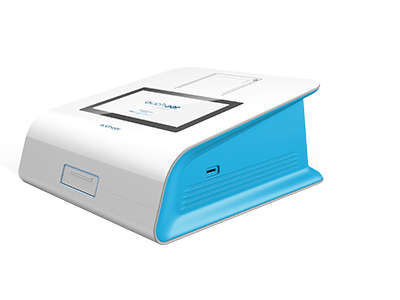
\includegraphics[width=.3\linewidth]{ch1/aocheng_kit}
    \caption{\label{fig:aocheng_kit}胎盘生长因子检测试剂盒}
\end{figure}
123

\subsubsection{1}

\subsection{人工智能技术}
今年来,由于计算机领域人工智能技术的高速发展,以及现代化设备的普遍使用,
相关研究者也开始尝试在子痫前期的识别、判断乃至预测等研究内容上引入人工智能技术。

\subsection{存在的不足与分析}
综合上述分析,对子痫前期的早期识别与检测可从按以下思路开展深入探索与研究。



\section{脉搏波在子痫前期领域研究现状}



\section{脉搏波时域特征研究现状}

\section{用脉搏波检测子痫的优势}
\section{研究目标与内容}

\subsection{研究目标}
\subsection{研究内容}

各章节的具体内容安排如下:

第一章是绪论。介绍子痫前期的定义及危害,梳理了目前临床已应用的检测方法及指标,分析各项方法的缺陷与不足。最后确定提出了本文的研究目标与内容。

第二章是子痫前期及光电容积脉搏波的生理学基础。

第三章是光电容积脉搏波的特征点检测算法。

第四章是光电容积脉搏波的特征集构建。

第五章是基于光电容积脉搏波特征的子痫前期检测识别模型。

第六章是低耦合高拓展的软件综合分析系统的设计与实现。

第七章是总结与展望。对本论文的全部研究工作进行系统性总结,阐述本论文的创新工作点,并对下一阶段的研究工作内容进行了规划与展望。


\chapter{生理学基础}
\section{引言}
由于本研究开展所使用的脉搏波数据均为通过光电容积描述标记的方法无创所得,因此在本章最后进一步阐述了微循环容积脉搏波血流模型及光电容积脉搏波采集原理。
\section{子痫前期的生理学基础}
\section{光电容积脉搏波概述}
\subsection{脉搏波产生原理}
\subsection{生理参数与非生理参数建立的心血管模型}
按照信号与系统的观点,若干相互作用、相互联系的事物按一定规律组成具有特定功能的整体均可称为系统,而信号则是反映信息的各种物理量,是系统直接进行加工、变换以实现通信的对象。而在脉搏波的工程研究领域,
人体的动脉管系亦可视为一个力学系统,心脏搏动作为该系统输入,而人体各处采集获得的脉搏波即为该系统输出(响应)。可由该系统的输入输出关系分析推断其结构特性参数,进一步研究脉搏波其他特性。\cite{PPGYY}

为尽可能精确描述心血管系统、探求心血管系统的生理特性,多年来学者们提出并建立了各种不同的数学模型进行拟合。而这些心血管模型大体上可依据建立时是否使用多个变量去拟合还原血液在血管中的可能涉及的血压、
血流弹性、阻力等生理变量分为生理参数模型与非生理参数模型两大类。\cite{PPGYY}生理参数模型关注心血管系统中的所有细节,模型中的各个参数变量均有较好的解释,也能与实际生理病理现象有较好的对应;而非生理参数则是
使用黑箱方法,不追求任何细节,仅通过输入输出信息来研究推导心血管系统模型,具有建立模型过程简单同时不破坏系统任何原有结构等优势。本节后续将分别从两大类模型中各选取一种经典模型进行介绍。
\subsubsection{双弹性腔模型}
\subsubsection{自回归平均移动模型}

\subsection{微循环容积脉搏波血流模型}

\subsection{光电容积脉搏波采集原理}
物理光学中,将光通过某种透明介质后被吸收的比例定义为光的吸收度$A$,即\autoref{equ:LBL}:
\begin{equation}
    \label{equ:LBL}
    A=\lg\frac{I_{0}}{I_{T}}
\end{equation}
其中,$I_{0}$与$I_{T}$分别是入射光强度与透射光强度。而朗伯-比尔定律(Lambert-Beer's law)指出,光的吸收度与入射光的强度无关,在光程上每等厚层介质吸收相同比例值的光,即\autoref{equ:LBL2}:
\begin{equation}
    \label{equ:LBL2}
    A=C \cdot \varepsilon \cdot V
\end{equation}
其中,$V$是透明介质的体积,$C$是透明介质的浓度,$\varepsilon$则是吸收系数,一般与透明介质的性质、入射光波长及温度等因素相关。

如图所示,在透射式的光电检测中考虑到人体指端各组织对入射光的均有吸收,以波长为$\lambda$的单色光垂直照射指端,则最终指端透射光强度为\autoref{equ:AF1}:
\begin{equation}
    \label{equ:AF1}
    I=I_{0}e^{-C_{t}\varepsilon _{t}V_{t}}e^{-C_{v}\varepsilon _{v}V_{v}} e^{-C_{a}\varepsilon _{a}V_{a}} 
\end{equation}
其中,下标$t$、$v$、$a$分别代表皮肤肌肉组织、静脉血液、动脉血液等成分。 学者们已经证实皮肤肌肉组织、静脉血液等组织对光的吸收是恒定不变的,同时若忽略由于散射、反射等因素造成的衰减,
则波长为$\lambda$的单色光垂直照射指端动脉血液,通过动脉血液的透光强度最终为\autoref{equ:AF2}:
\begin{equation}
    \label{equ:AF2}
    I=I_{0}e^{-C_{a}\varepsilon _{a}V_{a}} 
\end{equation}




\section{小结}


\chapter{脉搏波特征点检测算法}

\chapter{及特征参数集的构建}
\section{引言}
\section{信号预处理}
\section{脉搏波波形检测及纠错}
\section{时域特征参数设计与特征集构建}
\subsection{角度、幅值、长度等}
\section{小结}

\chapter{基于数据特征集的模型构建}
\section{引言}

\section{数据来源}
\section{构建方法分析}
\section{模型构建}
\section{小结}

\chapter{模型评估}
\section{引言}
\section{评估方式与标准}
\section{具体模型表现对比}
\section{小结}

\chapter{低耦合、高拓展的软件综合分析系统的设计与实现}
\section{背景分析}
* 子痫前期检测的特定场景:孕妇、高龄、周期长、时间

* 实验室已有前期硬件研究基础,家俊研究基础

\section{需求分析:模块化、低耦合、高拓展}
* 多场景

* 特征计算拓展

* 数据管理

* 模型识别判断

\section{整体设计框图展示}

\section{各模块具体设计}
* 硬件采集支持

* 对数据源的拓展——多种数据格式均可兼容

* 对数据预处理的拓展——波形定位算法可拓展、纠错算法可拓展

* 对数据类型的拓展——目前只涉及脉搏波,但可方便拓展ECG等信号

* 对特征集构建拓展——方便随时研发新的特征参数进入特征集

\section{实现展示与测试}
界面
输入输出
\section{小结}

\chapter{总结与展望}
\section{研究工作总结}
\section{主要创新点}
* 提出了多种新型脉搏波特征参数,从时域形态特征方面构建了一般通用的脉搏波特征集

* 从特征集中筛选出对子痫前期具有识别能力的有效特征集合,并基于有效特征集合通过机器学习方法构建了子痫前期综合预测模型

* 设计并实现了一种低耦合、高拓展的方便类似研究工作开展的软件综合分析系统

\section{下一阶段工作展望}


% \begin{algorithm}

% \end{algorithm}